\newcommand{\Goods}[1]{\index{#1}\index{Goods!#1}\hypertarget{#1}{\textbf{#1}}}
\newcommand{\Terrain}[1]{\index{#1}\index{Terrain!#1}\hypertarget{#1}{\textbf{#1}}}
\newcommand{\Unit}[1]{\index{#1}\index{Units!#1}\hypertarget{#1}{\textbf{#1}}}
\newcommand{\Building}[1]{\index{#1}\index{Buildings!#1}\hypertarget{#1}{\textbf{#1}}}
\newcommand{\Father}[1]{\index{#1}\index{Founding Fathers!#1}\hypertarget{#1}{\textbf{#1}}}
\newcommand{\FFather}[2]{\index{#2}\index{Founding Fathers!#2}\hypertarget{#1}{\textbf{#2}}}
\newcommand{\Report}[1]{\index{#1}\index{Reports!#1}\hypertarget{#1}{\textbf{#1}}}
\newcommand{\Concept}[1]{\index{#1}\hypertarget{#1}{\textbf{#1}}}
\newcommand{\Wikipedia}[1]{\href{http://en.wikipedia.org/wiki/#1}%
{
\includegraphics[scale=0.6]{images/wikipedia.png}}}

\documentclass[12pt]{article}
\usepackage{longtable}
\usepackage{graphicx}
\usepackage{index}
\usepackage[colorlinks=true,hyperindex=true]{hyperref}
\makeindex

\begin{document}
\author{\href{http://freecol.sourceforge.net/index.php?section=8}{The FreeCol Team}}
\title{FreeCol Documentation\\User Guide for Version v0.6.0}
\maketitle{}

\tableofcontents

\hypertarget{Introduction}{\section{Introduction}}

Welcome to FreeCol! If you're interested in development of this
program, please see the \href{http://freecol.sourceforge.net}{FreeCol
web site}. This is a draft version of the user's guide. You can find
the latest version at the
\href{http://freecol.sourceforge.net}{FreeCol homepage}.


\hypertarget{About}{\section{About}}

\hypertarget{About FreeCol}{\subsection{About FreeCol}}

The FreeCol team aims to create an Open Source version of
Colonization (released under the
\href{http://www.gnu.org/licenses/gpl.html}{GPL}). At
first we'll try to make an exact clone of Colonization. The visuals
will be brought up to date with more recent standards but will remain
clean, simple and functional. Certain new 'features' will be
implemented but the gameplay and the rules will be exactly the same as
the original game. Examples of modern features are: an isometric map
and multiplayer support.

This clone will be developed incrementally and result in
\textbf{FreeCol 1.0.0 which will be an almost exact Colonization
clone}. Incremental development basically means that we'll add
features one at a time. This allows us to have a running program at
all times and also to release an unfinished but working game once in a
while.

Once FreeCol 1.0.0 is finished we'll start working towards FreeCol
2.0.0. \textbf{FreeCol 2 will go beyond the original Colonization} and
will have many new features, it will be an implementation of our (and
our users') image of what Colonization 2 would have been.

\hypertarget{The Original Colonization}{\subsection{The Original Colonization}}

The original Colonization was released in 1994 by Microprose.
\textbf{Colonization is heavily based on Civilization} which is
generally considered to be the best turn-based strategy game for the
PC in the history of mankind.

In Civilization the object of the game was to build a nation that
could stand the test of times and that could also do one of the
following: conquer the world or be the first to launch a
spaceship. In Colonization things are bit different...

A Colonization game starts in 1492 and \textbf{the object of the game
is to colonize America}. You begin the game with one vessel and two
colonists.

As in Civilization you need to build a powerful nation, but
fortunately in the early part of the game \textbf{you'll be able to
send ships back to Europe} in order to sell the goods you've produced
or to bring back some colonists. \textbf{Getting colonists into the
new world is a very important aspect of the game} as one game turn
takes one year and later on even one season and as a result colonies
don't grow as rapidly as they do in Civilization. You can pay
colonists to come to the new world or you can show off with the
religious freedom of your people in which case they will hop on your
vessels for no money at all.

Another important aspect is \textbf{trade: the source of all income}
(apart from Inca and Aztec gold). In a land filled with precious
resources it is important to \textbf{build your colonies at the right
location} and to place crafstmen where they belong. This is not only
to have an income but also to be able to \textbf{live off the land}
when you can no longer count on the support of Europe.

Through all this you'll have to decide whether or not you want to
\textbf{live next to the native americans} peacefully. They can teach
your colonists new skills that cannot be tought anywhere else and they
will offer you goods in case you choose to treat them as your
friends. On the other hand, their villages can be attacked and their
valuable goods can be taken from them and sold in Europe.

\textbf{Other European forces are also busy occupying their piece of
the new world}. Should their borders go too far then take over some
of their colonies by force because they wouldn't hesitate to do the
same thing to you.

The object of Colonization is to \textbf{declare your independence and
survive an attack of the King's forces}. Before declaring your
independence \textbf{you need to have the majority of the people
behind you}. This can be done by \textbf{promoting free speech} and by
providing a strong governmental system.

\hypertarget{Installation}{\section{Installation}}

To compile FreeCol you'll need Java and the Ant build system. FreeCol
is known to work with Sun's Java 5, but not with projects based on GNU
Classpath, as some font handling classes used by FreeCol have not yet
been implemented. Ant can be found at \href{Ant
homepage}{http://ant.apache.org/}. FreeCol requires at least 128 MB
memory.

When these are installed, go to the root directory of FreeCol and type
\verb$ant$ to build a JAR file containing the game. The game is
started using the command \verb$java -Xmx128M -jar FreeCol.jar$.  If
something goes wrong, leave a bug report at the
\href{http://sourceforge.net/projects/freecol}{SourceForge page of
FreeCol}.

\hypertarget{Interface}{\section{Interface}}

This section will provide information about various interface
elements, as well as the keyboard shortcuts and the different actions
that can be used in the game.

\hypertarget{Starting the game}{\subsection{Starting the game}}

\hypertarget{Command line options}{\subsubsection{Command line options}}

First of all, you need to pass the Java Virtual Machine some arguments
that tell it how much memory to allocate and which jar file to open.
These are the arguments \verb$-Xmx128M$ and \verb$-jar FreeCol.jar$,
respectively. You can allocate more than 128 MB, if you like, but no
less. Refer to the manual of your Java Virtual Machine for details.

There are many other Java options, but you probably won't need to
change the default settings. FreeCol is developed in English, but it
includes translations into German, French, Spanish and Hungarian. Java
will automatically select the translation for your locale, if
available, and English otherwise. If you should wish to select a
language other than that associated with your locale, however, you can
do so by setting the system property values \verb$user.language$ and
\verb$user.country$ to the appropriate
\href{http://www.loc.gov/standards/iso639-2/php/code_list.php}{ISO
639} and
\href{http://www.iso.ch/iso/en/prods-services/iso3166ma/02iso-3166-code-lists/index.html}{ISO
3166} values. 

To use the French translation on a machine with a German locale, for
example, you need to specify \verb$-Duser.language=fr -Duser.country=FR$. 
You can also use environment variables to override
the locale, if your operating system supports that. To use the French
translation on a Linux system with a German locale, you could start
FreeCol like this, for example: \verb$LANG=fr_FR java -Xmx128M -jar FreeCol.jar$.

In addition to these general Java options, FreeCol also provides
several specific command line options:

\begin{itemize}
\item\verb$--freecol-data DIR$ Specify the directory that contains
FreeCol's data files. In general, you will not need to use this, as
the jar file contains all the necessary data files.
\item\verb$--windowed[[=]WIDTHxHEIGHT]$ Run FreeCol in windowed mode
instead of full screen mode and set the window width and height. You
will need this if your window manager does not (correctly support)
FreeCol's full screen mode. If you use Linux, for example, you should
set the window width to the width of your screen, but probably set the
window height slightly lower than the height of your screen, in order
to leave space for the menu bar, dock etc.
\item\verb$--load-savegame SAVEGAME_FILE$ Load the given
savegame. This is particularly useful in combination with the client
option \hyperlink{show savegame settings}{show savegame settings}.
\item\verb$--no-sound$ Run FreeCol without sound. Note that the game
does not yet contain any music, so the only sounds you will hear will
be special effects.
\item\verb$--usage$ Display the help screen.
\item\verb$--version$ Display the version number.
\item\verb$--server PORT$ Start a stand-alone server on the specifed
port. If you don't know what that means, you will not need the option.
\item\verb$--server-help$ Display a help screen for the more advanced
server options.
\end{itemize}

There are several other options that you will probably only be
intersted in if you are a developer:

\begin{itemize}
\item\verb$--no-java-check$ Skip the java version check.
\item\verb$--no-memory-check$ Skip the memory check.
\item\verb$--log-level LEVEL$ Set the java log level.
\item\verb$--debug$ Start the game in debugging mode.
\end{itemize}


\hypertarget{Game setup}{\subsubsection{Game setup}}

If you start FreeCol without command line options, the game will first
open a dialog that allows you to start a new game, to open a saved
game, to set various options, and to quit.

If you decide to start a new game, you will be presented with another
dialog, which enables you to start a single-player game, to retrieve a
list of servers from \verb$meta.freecol.org$\index{meta.freecol.org},
to join a \Concept{multi-player game}, or to start a new multi-player
game.

If you wish to join a multi-player game, you must enter the
\Concept{IP address} of a server that is running a FreeCol game as
well as the port it is running on. The default port is
$3541$\index{Port 3541}. If you wish to start a multi-player game,
then the IP address of the server will be that of your computer, but
you must still select a port to run the server on. Again, the default
port is $3541$. You must also decide whether you want to run a public
server or a private server. By default, you start a private game.

If you choose to retrieve a list of running games from the metaserver,
your computer will attempt to establish a connection to
\verb$meta.freecol.org$, port $3540$\index{Port 3540}. You will be
presented with a list of games, from which you can select one to
connect to. Please note that the list will frequently be empty, since
not that many public multi-player games are being run.

FreeCol is a client-server game. The game server takes care of the
game logic, and the client provides the graphical user interface. One
or several clients can connect to the game server via the network. In
the case of a single-player game, all other players are handled by the
game server. At the moment, however, your client uses a network
connection even if the server is running on the same computer.

This means that you can only run FreeCol if you have the necessary
privileges to bind an unprivileged port. If you use a
\Concept{personal firewall} that blocks the port you wish to use, you
will need to configure your firewall accordingly. If you wish to
retrieve a list of games from the metaserver, you also need to
configure your firewall to permit connections to that server, port
$3540$. In order to connect to a server, your client also needs to
bind a port. Which port depends on the operating system you use.


\hypertarget{Client options}{\subsection{Client options}}

The client options panel allows you to customize how your client
displays the game objects and how it handles some tasks such as
auto-saving.

First, we have general \hypertarget{display options}{display options}:

\begin{itemize}
\item The minimum number of goods to display with a counter. If you
accept the default setting of seven, for example, six hammers will be
diplayed without a number, and seven hammers will be displayed with
the number \verb$7$ on top. Note that many panels only show a single
item with a number next to it or below it anyway.
\item The maximum number of goods to display. If you accept the
default setting of seven, then no more than seven items will be
displayed, even if the corresponding counter tells you that these
seven items represent a far larger amount.
\item Whether to center on the active unit always.
\item Whether to display the Fog of War.
\item Whether to scroll the map when dragging with the mouse.
\item Whether to sort your colonies by name, age, position, size or
Sons of Liberty membership. Since name, age and position are unique,
these keys impose a total order, whereas size and Sons of Liberty
membership do not. In the case of size, the Sons of Liberty membership
is used as a secondary key, and vice versa.
\end{itemize}

Next, we have message display options: You can choose whether to group
messages by type, by source, or not at all. The source of the message
is a game object, typically a colony or unit, and the type of the
message is either the default type, which is always displayed, or one
of the following types, which can be turned off:

\begin{itemize}
\item Warning messages. These are important and should generally not
be turned off.
\item Messages about the Sons of Liberty membership in your colonies.
\item Messages about the efficiency of the government in your
colonies. The efficiency of the government influences the production
of all types of goods.
\item Messages about the number of goods in your colonies'
warehouses. 
\item Messages about units improving through experience, education or
promotion after a battle won.
\item Messages about units being demoted after a battle lost.
\item Messages about new units, such as colonists born in your
colonies.
\item Messages about units lost in battle, missing in action or dead
of starvation.
\item Messages about the completion of buildings in your colonies.
\item Foreign diplomatic messages about the declaration of wars and
signing of peace treaties.
\item Messages about the prices of goods in Europe changing.
\item Warnings about the suitability of prospective colony
sites. These messages are particularly useful for new players. Turn
them on if you are unsure where to establish your colonies.
\item Messages about the factors that influence combat. Turn them on
to learn more about things like the terrain bonus, the ambush bonus,
or the ``artillery in the open'' penalty.
\end{itemize}

Finally, there are the savegame settings:

\begin{itemize}
\item Whether to \hypertarget{show savegame settings}{show savegame
settings} always, only when starting multi-player games, or
never. These settings include the name, address and port of the game
server you wish to connect to. If you only play single-player games,
you can choose the option ``never''.
\item After how many terms you want the client to create an auto-save
file. If you select \verb$0$, then the client will never create
auto-save files.
\end{itemize}



\hypertarget{main screen}{\subsection{The main screen}}

The figure \ref{main_screen_fig} represents the main screen.
\begin{figure}[htb]
  \begin{center}
    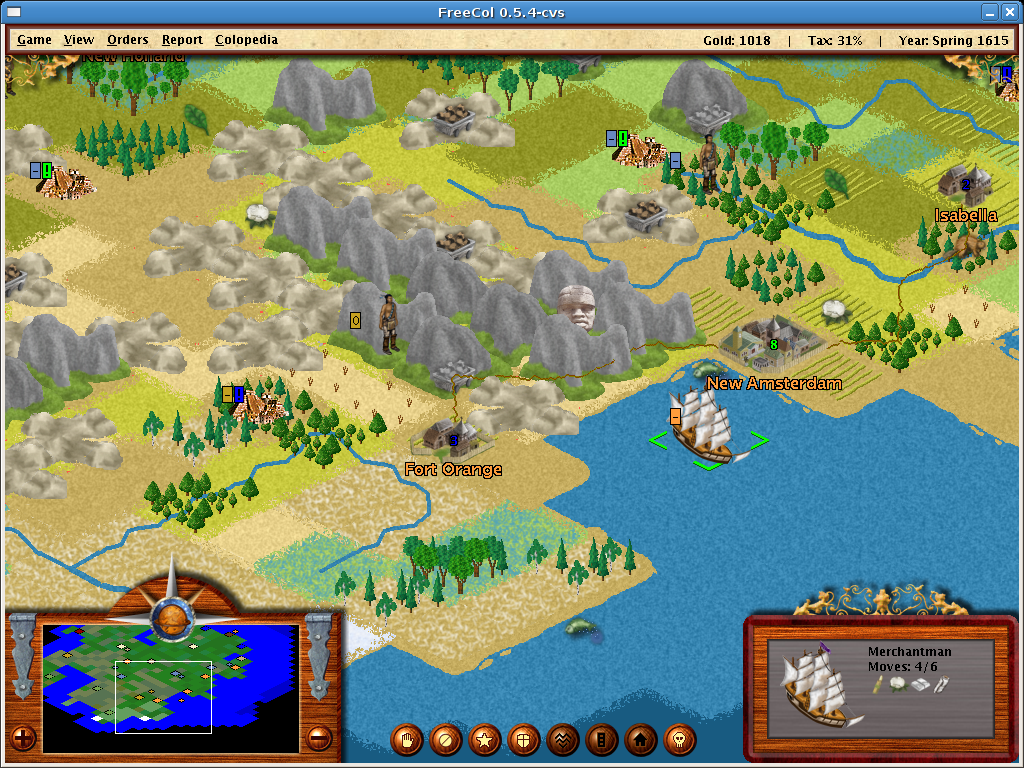
\includegraphics[scale=0.35]{images/main_screen.png}
    \caption{The main screen.\label{main_screen_fig}}
  \end{center}
\end{figure}

The main screen consists of five different areas: the menu bar at the
top, the minimap in the lower left corner, the info panel in the lower
right corner, the order buttons between the minimap and the info
panel, and the main map in the background. The units, colonies, and so
forth can be seen on the main map. They are also represented as
coloured dots on the minimap.

\hypertarget{menubar}{\subsubsection{The menubar}}

The menubar obviously contains the menu. It contains the submenus
Game, View, Orders, Report and Colopedia, at the left hand of the
screen, as well as a status area at the right hand of the screen. The
status area tells you about the amount of gold you possess, your
current tax rate and the current turn.

The \hypertarget{game menu}{Game Menu} allows you to:

\begin{itemize}
\item start a new game 
\item open a savegame
\item save the current game
\item change your preferences
\item reconnect to the server
\item chat with another player
\item declare independence
\item end your turn
\item quit
\end{itemize}

The \hypertarget{view menu}{View Menu} allows you to:

\begin{itemize}
\item turn the minimap and the info panel on or off
\item turn the display of tile names on or off
\item turn the display of tile owners on or off
\item turn the map grid on or off
\item switch between the unit view and the terrain view
\item switch to the Europe panel
\end{itemize}

The \hypertarget{orders menu}{Orders Menu} enables you to give orders
to the currently selected unit:

\begin{itemize}
\item wait until other units have moved
\item switch to sentry mode
\item fortify
\item go to a destination you select
\item build a colony
\item plow the tile the unit is on
\item build a road on the tile the unit is on
\item unload all goods and units on board
\item continue towards a selected destination
\item skip this turn
\item switch to a different unit on the same tile
\item forget current orders
\item change the unit's name
\item disband the unit
\end{itemize}

Note that not all orders are available at all times. The unload order
is only available if the unit is a carrier and is in a colony, for
example, and the build colony order is only available if the unit is
able to build colonies and the tile it is on will support a colony.

The \hypertarget{reports menu}{Reports Menu} provides access to
various reports on the current state of your colonies:

\begin{itemize}
\item The \Report{Religious Advisor} tells you how many crosses your
colonies produce, and how many crosses are required in order to
recruit the next emigrant in Europe.
\item The \Report{Labour Advisor} tells you which types of colonists
have emigrated to the New World or are waiting in Europe. If you can
not remember where you sent your only Expert Ore Miner, for example,
you can use this report to locate him.
\item The \Report{Colony Advisor} tells you which units are present in
each of your colonies, what each colony is producing, which buildings
have already been built, and which building is currently being built.
\item The \Report{Foreign Affairs Advisor} tells you about your
relations with foreign powers, the number of colonies and units they
possess, as well as their relative naval and military strength. As
soon as \hyperlink{Jan de Witt}{Jan de Witt} has joined the
\hyperlink{Continental Congress}{Continental Congress}, you are also
informed about the amount of gold, the number of Founding Fathers, the
current tax and the current Sons of Liberty membership of your
opponents.
\item The \Report{Indian Advisor} tells you about your relations with
the various Indian nations, and the number of settlements they
possess.
\item The \Report{Continental Congress Advisor} tells you which
Founding Fathers are already present in the \hyperlink{Continental
Congress}{Continental Congress} and which Founding Father is currently
being elected. It also tells you how many Liberty Bells each of your
colonies is producing, and whether they have already built the
\hyperlink{Printing Press}{Printing Press} and the
\hyperlink{Newspaper}{Newspaper}.
\item The \Report{Military Advisor} informs you of the deployment of
your military units, as well as the strength of the \hyperlink{Royal
Expeditionary Force}{Royal Expeditionary Force}.
\item The \Report{Naval Advisor} informs you of the whereabouts of
your naval units, as well as the strength of the \hyperlink{Royal
Expeditionary Force}{Royal Expeditionary Force}.
\item The \Report{Trade Advisor} details the current market prices of
all goods, the profits before and after taxes you have made, as well
as the amount of goods present in each of your colonies. Colonies that
have already built the \hyperlink{Custom House}{Custom House} are
highlighted, as are all goods that are currently being automatically
exported from these colonies.
\end{itemize}

The \hypertarget{colopedia menu}{Colopedia Menu} provides access to
the online game help, which is divided into six sections:

\begin{itemize}
\item The terrain section contains information on all the different
types of terrain you may encounter in the New World.
\item The unit section provides details on various types of units,
your own as well native units and units of the Royal Expeditionary
Force.
\item The goods section gives on overview of all the types of goods in
the game.
\item The building section provides information on the various
constructions you may build in your colonies.
\item The Founding Father section can be used to look up information
on the various Founding Fathers you may elect to the Continental
Congress.
\end{itemize}


\hypertarget{info panel}{\subsubsection{The Info Panel}}

The info panel in the lower right corner of the screen either shows
information on the currently selected unit, or contains a button to
end the current turn if no unit is selected. If a unit is selected,
then the info panel shows an image of the unit, as well as its name
and the moves it has left. If the unit is a carrier unit, such as a
ship or wagon train, the info panel also shows the units or goods on
board of the carrier. If the unit is a pioneer, the info panel shows
the number of tools the unit carries.


\hypertarget{minimap}{\subsubsection{The Minimap}}

The minimap in the lower left corner of the screen shows you a more
abstract view of the map than the main map. Different types of terrain
are distinguished by colour, and units and settlements are also
represented by dots in the colour of the nation that owns them. You
can use the minimap to navigate around the map quickly.  Either click
on the minimap to center the view on a certain point, or drag the
white frame around. Zoom buttons to the left and to the right of the
minimap allow you to zoom into and out of the view.


\hypertarget{unit buttons}{\subsubsection{The Unit Buttons}}

The unit buttons displayed between the minimap and the info panel
allow you to give order to your units. Note that not all buttons are
always active. A ship can not plow a tile, for example, so the plow
button is never active if the selected unit is a ship. The eight
buttons have the following functions:

\begin{itemize}
\item wait
\item skip turn
\item fortify
\item clear forest / plow tile
\item build road
\item build colony
\item disband unit
\end{itemize}

All these actions are also available from the \hyperlink{orders
menu}{Orders Menu} of the menu bar, and as \hyperlink{keyboard
shortcuts}{keyboard shortcuts}.


\hypertarget{main map}{\subsubsection{The Main Map}}

The main map shows you the New World in greater detail. You can see
the different types of terrain, forested and otherwise, hills,
mountains, rivers, and, of course, the various units and settlements
of the native and European players. Left click on a tile in order to
center the main map, or on a unit in order to select it (a
\hyperlink{display options}{display option} allows you to decide
whether the map should always centre on the selected unit, or
not). Left click on a colony in order to open the \hyperlink{colony
panel}{colony panel}. If there is an active unit outside of the colony
on the same tile, then a single left click will select the unit
instead. In this case, a double click will still open the colony
panel.

Right clicking on an empty tile, will either display some information
on that tile if no unit is selected, or open a pop-up menu that
additionally allows you to send the selected unit to this tile. If the
tile contains some of your units, the menu will also enable you to
select each of these units. If the tile contains a native settlement,
the menu will also provide you with an item that will bring up some
information on that settlement. It the tile contains one of your own
colonies, the menu will also allow you to open the \hyperlink{colony
panel}{colony panel}.

You can also activate the map scroll by moving the cursor towards the
edges of the main map. Scrolling with the minimap is faster, however.

If a unit is selected, further information about that unit is
displayed in the \hyperlink{info panel}{info panel}, and you can
\hypertarget{unit movement}{move the unit} using the numeric
keypad. If you select a unit with the left mouse button and drag the
mouse, the main map will display the best path from the unit's current
position to the tile the mouse is hovering over.

The tiles the path consists of will be marked with boots if the unit
is on foot, with horseshoes if the unit is mounted, with wheels if the
unit is a wagon train, or with sextants if the unit is a naval
unit. Full-colour symbols mark tiles that can be reached in the same
turn, whereas shaded symbols mark tiles that can be reached only in
subsequent turns. A number indicates how many turns later the unit
will arrive on this tile. 

  \begin{center}
    
\includegraphics{../data/images/ui/path-foot.png}
    
\includegraphics{../data/images/ui/path-horse.png}
    
\includegraphics{../data/images/ui/path-wagon.png}
    
\includegraphics{../data/images/ui/path-naval.png}
  \end{center}


Once you release the mouse button, the selected unit will begin to
follow this path. It will awake once it has arrived at its destination
or if it can no longer follow the path (if a unit belonging to a
different player is in the way, for instance). You can also press the
middle mouse button, or both mouse buttons if your mouse has two
buttons, in order to give the selected unit a movement order.

Units are marked with small coloured shields, which may or may not
display a letter. The background colour indicates the nation this unit
belongs to. The Dutch units, for example, are usually marked with
orange shields. The letter indicates the current state of the unit:

\begin{itemize}
\item\verb$-$: the unit is active (no orders).
\item\verb$F$: the unit is fortified.
\item\verb$G$: the unit is going somewhere.
\item\verb$P$: the unit is plowing a tile.
\item\verb$R$: the unit is building a road.
\item\verb$S$: the unit is a sentry.
\end{itemize}

If the unit is a foreign naval unit, the shield will display a number
instead. This is the number of holds this unit is using.

Indian Settlements display at least two shields: the first indicates
the nation this settlement belongs to, and the second, which bears an
exclamation mark ($!$), indicates the current relations between the
nation and your colonists. Its background may be green, blue, yellow,
orange or red, depending on whether your relations are good, mediocre
or bad. A Settlement with a European mission displays a third shield
bearing a cross on a black or grey background. The colour of the cross
indicates the European nation that established the mission. The
background of the shield is black if the mission was established by a
\hyperlink{Jesuit Missionary}{Jesuit Missionary}, and gray otherwise.

The order buttons represent some of the orders you can give to your
units. You can move your mouse over the buttons to see their
respective orders. If a unit is unable to perform a certain action,
the corresponding order button will be disabled. The orders are also
available from the \hyperlink{orders menu}{Orders Menu}, and you can
use the following \hypertarget{keyboard shortcuts}{keyboard shortcuts}:

\begin{itemize}
\item\verb$b$: build a colony.
\item\verb$c$: center on the currently selected unit.
\item\verb$d$: disband the active unit.
\item\verb$e$: show the Europe panel.
\item\verb$f$: fortify.
\item\verb$g$: goto some destination.
\item\verb$p$: plow the current tile.
\item\verb$r$: build a road on the current tile.
\item\verb$s$: sentry (not yet implemented).
\item\verb$w$: wait.
\item\verb$space$: skip for this turn.
\item\verb$enter$: end the turn.
\item\verb$plus$ or \verb$equals$: zoom in (not yet implemented).
\item\verb$minus$ or \verb$underscore$: zoom out (not yet implemented).
\item\verb$ctrl-d$: display tile names.
\item\verb$ctrl-g$: display grid.
\item\verb$ctrl-m$: show/hide the map controls.
\item\verb$ctrl-n$: new game.
\item\verb$ctrl-o$: open a game.
\item\verb$ctrl-q$: quit the game.
\item\verb$ctrl-r$: reconnect.
\item\verb$ctrl-s$: save a game.
\item\verb$ctrl-t$: show the chat panel.
\end{itemize}

\hypertarget{The Europe panel}{\subsection{The Europe panel}}

The figure \ref{europe_panel_fig} represents the Europe panel.
\begin{figure}[htb]
  \begin{center}
    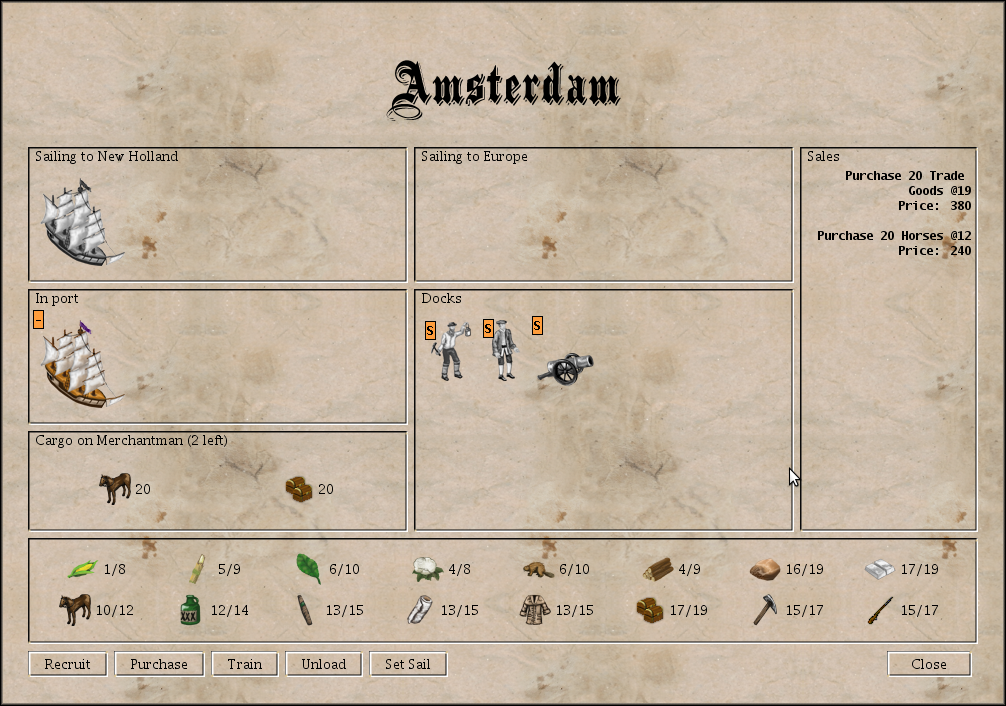
\includegraphics[scale=0.35]{images/europe_panel.png}
    \caption{The Europe Panel.\label{europe_panel_fig}}
  \end{center}
\end{figure}

In this panel, you can control the ships embarked for America or Europe,
and the ships currently stationed in Europe. You can also buy goods,
recruit, purchase and train units. Units recruited, purchased or trained
are in the �Docks� area in the Europe panel.

If a ship has set sail for Europe or America, you can change its
direction by dragging it from the �Going to America� box to the �Going
to Europe� box (or vice versa).

Ships that are docked at the European port can also do the following:
\begin{itemize}
\item Embark/Disembark units: drag and drop between the �Docks�
  and �Cargo� sections of the Europe panel.
\item Sell/Buy goods: drag and drop between the �Cargo� panel and the
  �Market� panel. If you want to sell only a part of your cargo, or
  want to buy less than 100 units of goods, press the shift key while
  dragging. This will allow you to specify how many units you wish to
  transfer. If any of the goods are displayed in grey, this means they
  are being boycotted by the Crown because you refused a tax
  raise. You must pay your tax arrears before you can trade these
  goods. You can do this by dragging the goods as usual, in which case
  you will be given the chance to pay your tax arrears (provided you
  have enough money).
\item Arm/Mount/Equip with tools/Dress as missionaries a unit: 
  right click on the unit.
\item Move your ship to the �Going to America� section of the Europe
  panel in order to sail to the New World.
\end{itemize}

\hypertarget{colony panel}{\subsection{The Colony panel}}

The figure \ref{colony_panel_fig} represents the Colony panel.
\begin{figure}[htb]
  \begin{center}
    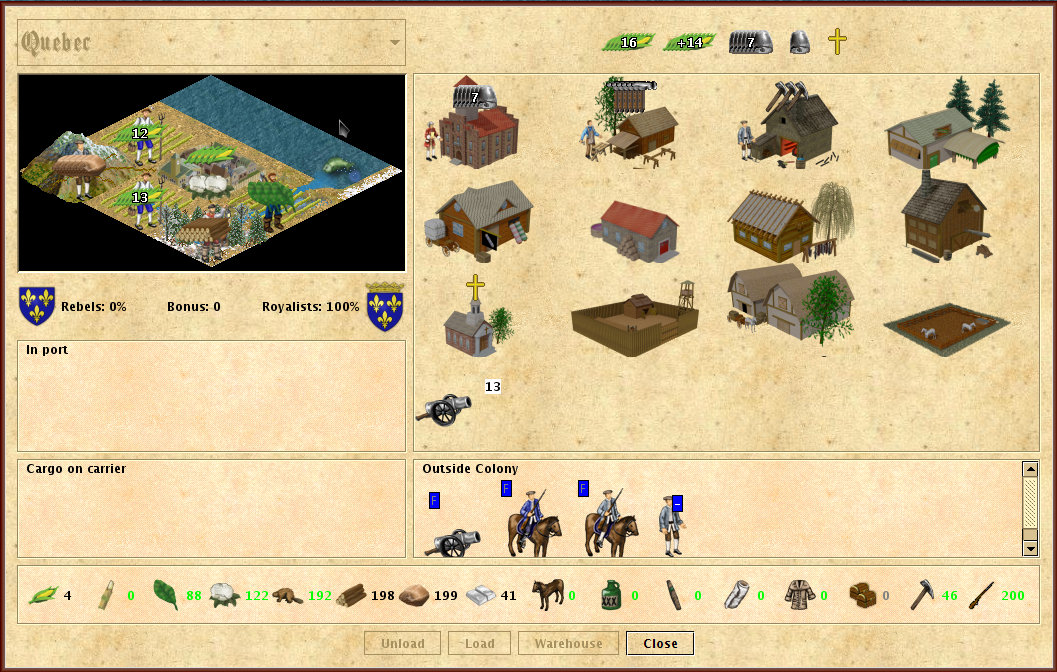
\includegraphics[scale=0.35]{images/colony_panel.png}
    \caption{The Colony Panel.\label{colony_panel_fig}}
  \end{center}
\end{figure}

To view a colony's panel, left click on it from the main
screen. From this panel, colonist's cultivation, production, and other
tasks can be assigned:

\begin{itemize}
\item Cultivation: Drop the unit onto the appropriate plot of land in
  the colony. You can change what a colonist cultivate by right
  clicking on it. Note that your colonists can not go fishing on ocean
  tiles before they have built \hyperlink{Dock}{Docks}.
\item Production: Drop the unit onto the relevant �Buildings�.
\item Depart colony: Drop the unit onto the colony's gate.
\item Embark on a ship: If there is a ship in port, you can embark
  your colonist on it by dropping it onto the �Cargo� section of the
  colony panel.
\item Build a building: Drop the unit onto the carpenter's house and
  select the building you want from the building menu.
\end{itemize}

You can also load a ship by dragging goods from the warehouse panel to
the ship, and unload it by dragging goods from the ship to the
warehouse panel. Use the shift key while dragging if you want to load
only a portion of the goods.

The \hyperlink{Warehouse}{Warehouse} can only hold a certain amount of
goods of each type. Its initial capacity is limited to 100 units of
each type of goods, but it can be increased to 300 by building two
\hyperlink{Warehouse Expansion}{Warehouse Expansions}. If the current
limit of the warehouse is exceeded, the number of goods is printed in
red. If you do not store the excess units elsewhere, they will be lost
at the end of the turn.

If you have already built a \hyperlink{Custom House}{Custom House} in
the colony, you can right-click on the goods in the Warehouse in order
to export them to Europe automatically. Goods marked to be exported
are printed in green. Right-click on the goods again to stop exporting
them automatically.


\hypertarget{The New World}{\section{The New World}}

At the beginning of the game, you will start with a naval vessel and
two colonists. Your first task will be to discover the New World,
which should lie due West, although sailing North or South may prove
quicker. As soon as you have discovered land, you can establish your
colonies and produce goods to send home to Europe.

\hypertarget{Terrain Types}{\subsection{Terrain Types}}

There are many different types of terrain in the New World, each with
its own peculiar advantages. At the beginning of the game you will
probably arrive at a \Terrain{High Seas} tile (or at the edge of the
map). High Seas tiles (and the map edge) allow you to sail between
Europe and the New World. As you approach land, the High Seas will be
replaced by \Terrain{Ocean} tiles, which produce
\hyperlink{Fish}{Fish}.

In the New World, you will also discover \Terrain{Plains}, which
produce a great deal of Grain, a lesser amount of Cotton, and some
Ore; \Terrain{Grassland}, on which Grain and Tobacco can be
cultivated; \Terrain{Prairie}, which are suitable for growing Grain
and Cotton; \Terrain{Savannah}, which produces Grain and Sugar;
\Terrain{Marsh}, where Grain can be cultivated and some Ore can be
mined; \Terrain{Swamp}, which yields some Grain, and small amounts of
Sugar, Tobacco and Ore; \Terrain{Desert}, which produce some Food,
Cotton and Ore; as well as \Terrain{Tundra}, where Grain can be grown,
and some Ore can be mined.

Large parts of the New World are covered in forests, all of which
yield varying amounts of Grain, Lumber and Furs. The \Terrain{Boreal
Forest} also produces Ore, the \Terrain{Mixed Forest} Cotton, the
\Terrain{Conifer Forest} Tobacco, the \Terrain{Tropical Forest} Sugar,
the \Terrain{Rain Forest} produces small amounts of Ore, Sugar and
Tobacco, the \Terrain{Wetland Forest} and the \Terrain{Scrub Forest}
yield some Ore, and the \Terrain{Broadleaf Forest} Cotton.

The \Terrain{Hills} produce a small amount of Grain, and can be mined
for Ore and a lesser amount of Silver. The \Terrain{Mountains} are
unsuitable for agriculture, but yield some Ore and Silver.
\Terrain{Arctic} tiles are the least useful type of terrain, as they
produce nothing at all. Terrain types that produce no Grain, such as
the Mountains and Arctic types, can not support colonies.

The New World is also irrigated by minor and major rivers. The
prouction of most types of \hyperlink{Goods}{Goods} is increased by
the presence of rivers and roads, which your
\hyperlink{Pioneer}{Pioneers} can build. All terrain types which
produce Grain (except the Hills) can also be cleared or plowed by your
Pioneers. In the case of open land, plowing increases the production
of Grain and most other types of goods. In the case of forests,
clearing removes the forest and transforms the tile into open land:
Boreal Forest is transformed into Tundra, Mixed Forest into Plains,
Conifer Forest into Grassland, Tropical Forest into Savannah, Wetland
Forest into Marsh, Rain Forest into Swamp, Scrub Forest into Desert,
and Broadleaf Forest into Prairie.


\hypertarget{Goods}{\subsection{Goods}}

The New World produces many goods, which can be traded in Europe.
Exporting these goods to Europe will be one of your most important
sources of income. At the beginning of the game, you will probably
want to export raw materials, such as \textbf{Sugar} and
\textbf{Tobacco}, but as prices drop, you should concentrate on luxury
products, such as \textbf{Rum} and \textbf{Cigars}, which command
higher prices.

\Goods{Food} is the single most important good, since all your
colonists consume two units of food each turn. If this demand can not
be met, some of your colonists will starve to death.  On the other
hand, a colony that has accumulated 200 units of food will produce a
new \hyperlink{Free Colonist}{Free Colonist}.  Buying food in Europe
is always expensive, but unfortunately colonial foodstuffs fetch only
poor prices.

Food comes in two varieties, \Goods{Grain}, which can be cultivated on
nearly all land tiles, and \Goods{Fish}, which is produced by
\hyperlink{Ocean}{ocean} and lake tiles. In order to harvest the
bounty of the sea, you will need a \hyperlink{Dock}{Dock}, however.

Breeding new \Goods{Horses} also requires food, but the horses you
already have are content to eat grass and consume no more of your
precious food. Breeding horses does not require
\hyperlink{Stables}{Stables}, but Stables do speed things up.

Four raw materials are typical for the New World. They will initially
generate a good income, but prices will inevitably drop. These goods
are \Goods{Sugar}, which is best cultivated on
\hyperlink{Savannah}{Savannah} tiles, \Goods{Tobacco}, best cultivated
on \hyperlink{Grassland}{Grassland}, \Goods{Cotton}, which is most
abundant on \hyperlink{Prairie}{Prairie} tiles, and \Goods{Furs},
which are available on all forested tiles, but most abundantly on
\hyperlink{Boreal Forest}{Boreal Forest} and \hyperlink{Mixed
Forest}{Mixed Forest} tiles.

These four materials can be used to produce corresponding luxury
goods, which will fetch much higher prices in Europe. In a
\hyperlink{Distiller's House}{distillery}, \Goods{Rum} is produced
from Sugar. Tobacco is used to make \Goods{Cigars} in the
\hyperlink{Tobacconist's House}{Tobacconist's House}. The Weaver
weaves \Goods{Cloth} from Cotton in his \hyperlink{Weaver's
House}{house}, and the Fur Trader turns Furs into \Goods{Coats} in his
\hyperlink{Fur Trader's House}{house}.

Initially, the resource which fetches the highest prices in Europe is
\Goods{Silver}, which can be mined in \hyperlink{Hills}{Hills} and
\hyperlink{Mountains}{Mountains}. As prices drop, Silver will become
less and less useful, however. On the other hand, Hills and Mountains
also produce \Goods{Ore}, which is not in great demand in Europe, but
which can be refined to produce \Goods{Tools} in the
\hyperlink{Blacksmith's House}{Blacksmith's House}. Tools are required
for clearing forests and plowing fields, as well as for constructing
advanced buildings and units. Furthermore, \Goods{Muskets} can be
produced from Tools in the \hyperlink{Armory}{Armory}.

\Goods{Lumber} also fetches poor prices in Europe, but can be used to
produce \Goods{Hammers} in the \hyperlink{Carpenter's
House}{Carpenter's House}. Hammers are required for constructing all
buildings, as well as \hyperlink{Naval Units}{naval units} and
\hyperlink{Wagon Train}{Wagon Trains}. Hammers are ``abstract'' goods
that can neither be transported nor traded. They represent the work
required to finish a building rather than some tangible material.

The two other ``abstract'' goods are \Goods{Liberty Bells}, which are
produced in the \hyperlink{Town Hall}{Town Hall}, and \Goods{Crosses},
which are generated by the \hyperlink{Church}{Church}. They represent
the concepts of liberty and of religious freedom. Liberty Bells are
needed to convince your colonists of your policies, and to elect
\hyperlink{Founding Fathers}{Founding Fathers} to the
\hyperlink{Continental Congress}{Continental Congress}, whereas
Crosses attract further colonists.

\Goods{Trade Goods}, on the other hand, can be transported and traded,
but they can not be produced in your colonies. They are only available
in Europe and are useful for trading with native settlements, which
generally demand Trade Goods.


%% \hypertarget{Resources}{\subsection{Special Resources}}

%% Some types of terrain can also have special resources, which increase
%% the production of one or more types of goods.


\hypertarget{Native Settlements}{\subsection{Native Settlements}}

The New World is by no means an uninhabited country. Various tribes of
Indians already live there, and make use of the land. When your
colonists arrive, you will have to decide whether you will attempt to
peacefully coexist with the natives, or to wipe them out. The
\hyperlink{France}{French} player has the advantage of generating only
half the alarm among the natives. The \hyperlink{Spain}{Spanish}
player has the advantage of greater military efficiency against the
natives. Your choice of \hyperlink{Home Country}{Home Country} may
influence your strategy --- or vice versa.

Small Native Settlements use the tile they are built on as well as all
adjacent tiles, just like your \hyperlink{Colonies}{Colonies}
do. Large Native Settlements also use tiles that are two moves
away. Your colonists can not use tiles that are already used by
natives. If they attempt to do so, the natives will demand some gold
for the land. You must then decide whether to pay their price, take
the land away from the by force, or to leave the land alone.
Naturally, the natives will not be pleased if you take the land away
from them. As soon as \hyperlink{Peter Minuit}{Peter Minuit} has
joined the \hyperlink{Continental Congress}{Continental Congress},
however, the natives no longer demand payment for their land.

Colonies and armed units near their settlements will alarm the natives
and poison your relations. If the natives are happy, they will come to
your colonies offering gifts. If they are unhappy, they will come and
make demands instead. If they get really angry, they may attack your
units or colonies. After a few turns, however, they will usually calm
down again.

Some types of units may enter Native Settlements. Units that carry
goods, such as \hyperlink{Wagon Train}{Wagon Trains} and
\hyperlink{Naval Units}{Ships}, can enter the settlements and trade
with them. Trade always improves your relations with the natives.

\hyperlink{Scout}{Scouts} can either demand tribute, or ask to speak 
with the chief of the tribe. Demanding tribute is obviously not good
for your relations with the natives, whereas speaking with the chief
for the first time may be to your advantage. The chief may offer you
some gold, or tell you about nearby lands. If your Scout is not a
\hyperlink{Seasoned Scout}{Seasoned Scout} already, he may become so.

\hyperlink{Free Colonist}{Free
Colonists} and \hyperlink{Indentured Servant}{Indentured Servants} may
enter a settlement in order to learn the skills of the natives. And
\hyperlink{Missionary}{Missionaries}, which may be either
\hyperlink{Jesuit Missionary}{Jesuit Missionaries} or ordinary
colonists blessed as missionaries in the \hyperlink{Home Port}{Home
Port} or any colony with a \hyperlink{Church}{Church}, are able to
establish a \Concept{Mission} or to incite the natives against another
European nation.

The presence of a Mission will reduce tension between the natives and
your colonists. In time, some of the natives may also convert and join
your colonies as \hyperlink{Indian Convert}{Indian Converts}.


\hypertarget{Lost City Rumours}{\subsection{Lost City Rumours}}

In the New World, there are also rumours about \Concept{Lost Cities},
such as El Dorado, or C{\'\i}bola. You may send your colonists to
explore these rumours, and you might indeed discover one of the Seven
Cities of Gold, and a \hyperlink{Treasure Train}{Treasure Train}.
Other outcomes, however, are also possible.

Mostly, the rumour proves to be nothing but a rumour. Occasionally,
you might disturb the burial grounds of a native tribe, which will
cause the tribe to declare war on you. It is also possible that your
expedition simply vanishes without a trace. On the other hand, you
might also discover a small tribe and a few trinkets. Your colonist
might become a \hyperlink{Seasoned Scout}{Seasoned Scout} if he has no
other skill, or you might discover the sole survivor of a lost
colony.

Possibly the best outcome is the discovery of the \Concept{Fountain of
Youth}, which will cause numerous colonists to appear on the docks in
your \hyperlink{Home Port}{Home Port}.

As soon as \hyperlink{Hernando de Soto}{Hernando de Soto} has joined
the \hyperlink{Continental Congress}{Continental Congress}, Lost City
Rumours always yield positive results.


\hypertarget{Colonies}{\section{Colonies}}

\hypertarget{Picking a suitable site}{\subsection{Picking a suitable site}}

Your colonies are your most important assets in the new world.
Therefore, it is very important to build them in the right
place. There are several aspects to consider:

\hypertarget{The colony tile}{\subsubsection{The colony tile}}

Some terrain types are more suitable for establishing a colony than
others. Colonies can not be built on Arctic tiles, nor on Mountains,
because these terrain types produce no Grain. Hills and Deserts are
less suitable than other tiles because they produce less food, which
is very important in the long run. Tiles with forest generally produce
less food than tiles without, but \hyperlink{Pioneer}{Pioneers} are
able to cut down the forest and plow the tile, which will increase
food production. The presence of a river will also increase food
production.

The \hyperlink{Hills}{Hills} produce a small amount of Grain, and can
be mined for Ore and a lesser amount of Silver. The
\hyperlink{Mountains}{Mountains} are unsuitable for agriculture, but
yield some Ore and Silver. \hyperlink{Arctic}{Arctic} tiles are the
least useful type of terrain, as they produce nothing at all. Terrain
types that produce no Grain, such as the Mountains and Artic types,
can not support colonies.

The New World is also irrigated by minor and major rivers. The
prouction of most types of \hyperlink{Goods}{Goods} is increased by
the presence of rivers and roads, which your
\hyperlink{Pioneer}{Pioneers} can build. All terrain types which
produce Grain (except the Hills) can also be cleared or plowed by your
Pioneers. In the case of open land, plowing increases the production
of Grain and most other types of goods. In the case of forests,
clearing removes the forest and transforms the tile into open land:
Boreal Forest is transformed into Tundra, Mixed Forest into Plains,
Conifer Forest into Grassland, Tropical Forest into Savannah, Wetland
Forest into Marsh, Rain Forest into Swamp, Scrub Forest into Desert,
and Broadleaf Forest into Prairie.


\hypertarget{The adjacent tiles}{\subsubsection{The adjacent tiles}}

In the early stages of the game, you will need to generate cash by
selling products from the New World in your Home Port. Thus, many of
your early colonies should probably be situated next to bonus tiles,
which greatly increase production. Rivers also increase production,
though not as much as a bonus resource. On the other hand, they
increase the production of many different kinds of goods, unlike a
bonus resource.

In order to improve your colony, you will have to construct various
buildings. This will require large amounts of lumber. For this reason,
you should make sure that at least one tile adjacent to your colony
site can produce sufficient amounts of lumber. You will also need
tools to construct advanced buildings. Therefore, it is an advantage
if the colony can also produce ore, which can be refined to produce
tools. However, ore is not as important as lumber.

Some of the tiles may be owned by other European powers, or claimed by
Indians. Building a colony too close to other settlements is not a
good idea, unless you plan to conquer or destroy these settlements.
But remember that colonies with a \hyperlink{Stockade}{Stockade} can
not be abandoned.  Keeping your own colonies close together is a good
strategy, however, as long as you avoid sharing tiles between several
colonies as far as possible.

\hypertarget{No Reforestation}{\subsubsection{No Reforestation}}

You can order your pioneers to cut down forests by plowing a tile.
This will increase the food produced on these tiles, and the lumber
will be delivered to your colonies. However, you can not plant new
forests later. Once cleared, a tile will never produce lumber again.

\hypertarget{Colony Buildings}{\subsection{Colony Buildings}}

A newly established colony already includes several buildings, namely
a town hall, a carpenter's house, a blacksmith's house, a
tobacconist's house, a weaver's house, a distiller's house, a fur
trader's house, and a warehouse. You can improve your colonies by
upgrading all of these buildings except the town hall, and by
constructing various new buildings. However, many buildings can only
be constructed in colonies of a certain size, or after certain
\hyperlink{Founding Fathers}{Founding Fathers} have joined the
\hyperlink{Continental Congress}{Continental Congress}.

The craftsmen's houses can be upgraded to workshops, which produce
more manufactured goods. After \hyperlink{Adam Smith}{Adam Smith} has
joined the \hyperlink{Continental Congress}{Continental Congress},
workshops can be upgraded to factories, which produce one and a half
units of manufactured goods from each unit of raw material. While the
town hall itself can not be upgraded, the production of
\hyperlink{Liberty Bells}{Liberty Bells} can be boosted by
constructing a printing press and then a newspaper.

All in all, there are sixteen different buildings, eight of which are
part of every newly established colony:

\begin{itemize}
\item The \Building{Town Hall}, which can not be upgraded, provides
  workplaces for up to three colonists producing \textbf{Liberty
  Bells}. Its effect can be increased by building a
  \hyperlink{Printing Press}{Printing Press} and a
  \hyperlink{Newspaper}{Newspaper}.

\item The \Building{Carpenter's House}, which can be upgraded to a
  \textbf{Lumber Mill} once the colony's population reaches 3, is used
  to convert \hyperlink{Lumber}{Lumber} to
  \hyperlink{Hammers}{Hammers}. Hammers are required to construct or
  upgrade all kinds of buildings.

\item The \Building{Blacksmith's House}, which can be upgraded to a
  \Building{Blacksmith's Workshop}, is used to convert
  \hyperlink{Ore}{Ore} to \hyperlink{Tools}{Tools}. Tools are required
  to construct certain kinds of buildings and to upgrade all kinds of
  buildings. Tools are also used by \hyperlink{Pioneer}{Pioneers} and
  to produce \hyperlink{Muskets}{Muskets}. Once the population of the
  colony has reached 8, the Blacksmith's Workshop can be replaced by
  \Building{Iron Works}, provided that \hyperlink{Adam Smith}{Adam
  Smith} has joined the \hyperlink{Continental Congress}{Continental
  Congress}.

\item The \Building{Tobacconist's House}, which can be upgraded to a
  \Building{Tobacconist's Shop}, is used to produce
  \hyperlink{Cigars}{Cigars} from \hyperlink{Tobacco}{Tobacco}.  Once
  the colony's population has reached 8, it can be further upgraded to
  a \Building{Cigar Factory}, provided that \hyperlink{Adam
  Smith}{Adam Smith} has joined the \hyperlink{Continental
  Congress}{Continental Congress}.

\item The \Building{Weaver's House}, which can be upgraded to a
  \Building{Weaver's Shop}, is used to turn \hyperlink{Cotton}{Cotton}
  into \hyperlink{Cloth}{Cloth}. It can be upgraded to a
  \Building{Textile Mill} as soon as the population of the colony is
  at least 8 and \hyperlink{Adam Smith}{Adam Smith} has joined the
  \hyperlink{Continental Congress}{Continental Congress}.

\item The \Building{Distiller's House}, which can be upgraded to a
  \Building{Rum Distillery}, is used to produce \hyperlink{Rum}{Rum}
  from \hyperlink{Sugar}{Sugar}. Once \hyperlink{Adam Smith}{Adam
  Smith} has joined the \hyperlink{Continental Congress}{Continental
  Congress} and the colony's population is at least 8, the rum
  distillery can be replaced by a \Building{Rum Factory}.

\item The \Building{Fur Trader's House}, which can be upgraded to a
  \Building{Fur Trader's Post}, is used to produce
  \hyperlink{Coats}{Coats} from \hyperlink{Furs}{Furs}. Once the
  colony's population has reached 6, it can be further upgraded to a
  \Building{Fur Factory}, provided that \hyperlink{Adam Smith}{Adam
  Smith} has joined the \hyperlink{Continental Congress}{Continental
  Congress}.

\item The \Building{Warehouse} stores all kinds of goods. Its initial
  capacity is 100 units of each kind of goods, but it can be upgraded
  to a \Building{Warehouse Expansion}, which holds 200 and finally 300
  units.
\end{itemize}

The following eight buildings are not part of your basic colony and
have to be constructed later:

\begin{itemize}
\item A colony with a population of at least 4 may build a
  \Building{Schoolhouse}, which enables some master craftsman to teach
  an unskilled colonist their trade. As soon as the population reaches
  8, it can be upgraded to a \Building{College}, in which additional
  trades can be taught by two colonists. Once the population reaches
  10, the college can be replaced by a \Building{University}, at which
  all trades can be taught by three colonists. See \hyperlink{Skills
  and Education}{Skills and Education} for details.

\item The \Building{Armory} is used to produce
  \hyperlink{Muskets}{Muskets} from \hyperlink{Tools}{Tools}. As soon
  as the population reaches 8, the armory can be upgraded to a
  \Building{Magazine} and then to an \Building{Arsenal}, provided that
  \hyperlink{Adam Smith}{Adam Smith} has joined the
  \hyperlink{Continental Congress}{Continental Congress}.

\item A colony with a population of 3 or more may build a
  \Building{Church}, which can be upgraded to a \Building{Cathedral}
  as soon as the population reaches 8. The religious freedom of the
  New World (symbolized by \hyperlink{Crosses}{Crosses}) causes
  increased emigration from Europe.

\item The \Building{Stockade}, which can be constructed as soon as the
  colony's population reaches 3, protects the colonists from
  attacks. Note that a colony with a stockade can not be abandoned, it
  can only be burned to the ground by natives. The stockade can be
  upgraded to a \Building{Fort}, which provides better protection and
  bombards \hyperlink{Privateer}{Privateers} and enemy naval units on
  adjacent ocean tiles. The fort can be replaced by a
  \Building{Fortress} as soon as the population reaches 8.

\item The \Building{Stables} increase the production of
  \hyperlink{Horses}{Horses}.

\item The \Building{Dock} allows colonists to produce
  \hyperlink{Fish}{Fish} on ocean tiles adjacent to the colony. As
  soon as the population is at least 4, it can be upgraded to a
  \Building{Drydock}, which allows the colony to repair damaged
  ships. When the colony's population reaches 8, it can be further
  upgraded to a \Building{Shipyard}, which enables the colony to build
  new ships.

\item The \Building{Printing Press}, which can be upgraded to a
  \Building{Newspaper} as soon as the population reaches 4, increases
  the colony's production of \hyperlink{Liberty Bells}{Liberty Bells}.

\item The \Building{Custom House}, which can
  be built as soon as \hyperlink{Peter Stuyvesant}{Peter Stuyvesant}
  has joined the \hyperlink{Continental Congress}{Continental
  Congress}, allows the colony to export goods to Europe directly
  without the help of ships. Optionally, it may also ignore
  \hyperlink{Boycotts}{Boycotts}.

\end{itemize}


\hypertarget{Home Country}{\section{Your Home Country}}

Your \textbf{Home Country} is a European monarchy, either 
\Concept{Spain}, \Concept{France}, \Concept{England} or the 
\Concept{Netherlands}\index{Dutch}. Each of these countries has one
special ability. If you hail from Spain, you will be more successful
fighting against the natives. If you are French, you will be more
successful cooperating with the natives. The English generate more
colonists, and the Dutch are better traders.

\hypertarget{Home Port}{\subsection{Your Home Port}}

The \textbf{Home Port} is a port city in your home country, where you
can trade \hyperlink{Goods}{Goods}, and train, recruit and buy
\hyperlink{Units}{Units}. If you have not built a
\hyperlink{Drydock}{Drydock} in any of your colonies, your damaged
ships will also return to the Home Port for repairs.

As you generate \hyperlink{Crosses}{Crosses} in your colonies,
colonists will appear at the docks of the Home Port. Unless
\hyperlink{William Brewster}{William Brewster} has joined the
\hyperlink{Continental Congress}{Continental Congress}, many of these
colonists will be \hyperlink{Indentured Servant}{Indentured Servants}
and \hyperlink{Petty Criminal}{Petty Criminals}. Once William
Brewster has been elected, these units will no longer appear at the
docks, and you will be able to select the next colonist to emigrate
from the recruitment list.

The recruitment list is a list of three colonists who are thinking
about emigrating to the New World, but have not yet reached a
decision. You can recruit them by offering gold as an incentive. At
the beginning of the game, this is a good way of increasing the
population of your colonies. However, the amount of gold required will
greatly increase during the game.

If you have enough gold, you can also train colonists at the
\hypertarget{Royal Academy}{Royal Academy}. In exchange for the
education you provide, they will also emigrate to the New World. Not
all types of colonists can be trained at the Royal Academy, however.

\hyperlink{Naval Units}{Ships} and \hyperlink{Artillery}{Artillery}
can also be purchased in the Home Port. You can also build these units
in your colonies, as soon as you have built a
\hyperlink{Shipyard}{Shipyard} and an \hyperlink{Armory}{Armory},
respectively.


\hypertarget{Monarch}{\subsection{Your Monarch}}

Your Home Country is ruled by a \textbf{Monarch} whose actions can
have a profound influence on your colonies and your relations to other
nations present in the New World. 

From time to time, the Monarch may decide to raise the
\Concept{Taxes}{Taxes} you pay on all goods you sell in the Home
Port. You may refuse to accept these taxes, however, in which case
your colonists will stage a protest similar to the \Concept{Boston Tea
Party} and throw some goods into the harbour. The Monarch will not be
amused and will \index{Boycotts} \hypertarget{Boycotts}{boycott} this
type of goods. This means that you will no longer be able to trade
these goods in the Home Port until the Boycott is lifted.

You can end a Boycott by paying the outstanding tax arrears. As soon
as \hyperlink{Jacob Fugger II} joins the \hyperlink{Continental
Congress}{Continental Congress}, all Boycotts will be lifted, but the
Monarch may declare further Boycotts later on. As soon as
\hyperlink{Peter Stuyvesant} joins the \hyperlink{Continental
Congress}, you will be able to build \hyperlink{Custom House}{Custom
Houses} in your colonies. The original Colonization game contained a
bug which made the Custom House ignore all Boycotts, and this
behaviour is available as a rule variant.

Naturally, the Monarch does not trust your colonists, some of which
are nothing but \hyperlink{Petty Criminal}{Petty Criminals}, and some
of which even support the infamous \hyperlink{Sons of Liberty}{Sons of
Liberty}. For this reason, the crown maintains the
\Concept{Royal Expeditionary Force}, which is to put an end to
insurrections in the New World. From time to time the Monarch may
inform you that further units have been added to the Royal
Expeditionary Force, just so that you don't get any ideas.

The Monarch may also declare war on any nation present in the New
World, both European and native. This will also affect your relations
with this nation, unless \hyperlink{Benjamin Franklin}{Benjamin
Franklin} has already been elected to the \hyperlink{Continental
Congress}{Continental Congress}. In this case, the Monarch's wars do
not affect you anymore.

If you are already at war with some nation, either due to the
Monarch's actions, or your own, the crown may offer you some cheap
\Concept{Mercenaries}. If you agree to their price, these units will
appear at the docks in your Home Port, ready to set sail for the New
World.



\hypertarget{Units}{\section{Units}}

Several dozen different units are available in FreeCol, but not all
units are available to all players. Some units are available only to
\textbf{Indian Players}, some units are only available to
\textbf{European Players}, and other units are available only to the
\textbf{Royal Expeditionary Force}.

The most basic unit of the European Players (including you) is the
\Unit{Free Colonist}. The Free Colonist is quite good at any task, but
has no special skills. At the beginning of the game, many of the
colonists will not be volunteers, but \Unit{Indentured Servant}, or
\Unit{Petty Criminal}, who are deported to the New World. Indentured
Servants are pretty bad at all jobs within the colony, but just like
Free Colonists, they can be sent to native villages to learn a skill
from the natives. Petty Criminals are very bad at all jobs within the
colony and can not learn anything from the natives. However, both
Indentured Servants and Petty Criminals can become Free Colonists
through \hyperlink{Skills and Education}{Education}.

Many early colonies failed due to a lack of food. In order to avoid a
similar fate, you must ensure adequate food production from the very
beginning. All your colonists can produce some amount of food,
especially on the more fertile terrain types, but \Unit{Expert Farmer}
and the \Unit{Expert Fisherman} will greatly increase your food
production. But note that the Expert Fisherman requires a
\hyperlink{Dock}{Dock} to moor his boat to, and that this requires at
least one ocean tile adjacent to your colony.

Three types of units are not available in Europe because they posses
skills that can only be learned from the native population. These are
the \Unit{Master Sugar Planter}, the \Unit{Master Cotton Planter}, the
\Unit{Master Tobacco Planter}, and the \Unit{Expert Fur
Trapper}. These units are able to greatly increase your production of
\hyperlink{Sugar}{Sugar}, \hyperlink{Cotton}{Cotton},
\hyperlink{Tobacco}{Tobacco}, and \hyperlink{Furs}{Furs},
respectively.

In the beginning of the game, you will most likely export a great deal
of these goods to Europe, but beware, prices will drop! However, all
the raw materials of the New World can be used to produce luxury goods
that will sell for higher prices in Europe. \hyperlink{Sugar}{Sugar}
can be used to distill \hyperlink{Rum}{Rum},
\hyperlink{Cotton}{Cotton} can be used to produce
\hyperlink{Cloth}{Cloth}, \hyperlink{Cigars}{Cigars} are made from
\hyperlink{Tobacco}{Tobacco}, and \hyperlink{Coats}{Coats} are made
from \hyperlink{Furs}{Furs}. All your colonists can do this, but the
\Unit{Master Distiller}, the \Unit{Master Weaver}, the \Unit{Master
Tobacconist}, and the \Unit{Master Fur Trader} are the experts who
will really rev up your production.

The New World also has two mineral resources, \hyperlink{Ore}{Ore} and
\hyperlink{Silver}{Silver}, to offer. Again, all your colonists are
able to mine these resources to a certain extent, but you will need
the \Unit{Expert Ore Miner} and the \Unit{Expert SilverMiner} to make
the most of them.

\hyperlink{Lumber}{Lumber} can be produced in all forested tiles, and
can also be exported to Europe, although prices are low. However, you
will need vast amounts of lumber in order to upgrade your colonies,
and no colonist is more skilled at cutting down forests than the
\Unit{Expert LumberJack}. Nor is any colonist more skilled at turning
the lumber into buildings than the \Unit{Master Carpenter}.

The more advanced buildings you can construct in the your colonies
require not only lumber but also \hyperlink{Tools}{Tools}, which are
produced from \hyperlink{Ore}{Ore}. This is the job the \Unit{Master
Blacksmith} excels in.  Tools are also used by your \Unit{Pioneer} to
clear forests and plow fields, but none of your other colonists can
match the outdoors skills of your \Unit{Hardy Pioneer}. And finally,
Tools are required for the production of \hyperlink{Muskets}{Muskets},
a demanding task best left to the \Unit{Master Gunsmith}.

All your units are able to explore the New World, but the colonist
most suited to this dangerous endeavour is the \Unit{Scout}, a mounted
colonist. A Scout may become a \Unit{Seasoned Scout} through
\hyperlink{Skills and Education}{experience}, either by visiting
native settlements, or by investigating \hyperlink{Lost City
Rumours}{Lost City Rumours}. The Seasoned Scout is much more skillful
at these jobs, but beware, they are dangerous!

Another colonist able to visit native settlements is the
\Unit{Missionary}. Any colonist can be converted to a Missionary by
blessing him in a colony with a \hyperlink{Church}{Church}, or in the
\hyperlink{Home Port}{Home Port}, which is sure to have several
churches and maybe even a
\hyperlink{Cathedral}{Cathedral}. Missionaries are able to establish a
\hyperlink{Mission}{Mission} in the native settlement, and to convert
the natives. The \Unit{Jesuit Missionary}, however, is much more
accomplished at the job.

The converted natives may join your colonies as \Unit{Indian
Convert}. They are unskilled at all jobs within the colony, but more
skilled than your Free Colonists at all outdoor jobs. Indian Converts
can not be upgraded through \hyperlink{Skills and
Education}{Education}, but they become Free Colonists as soon as
\hyperlink{Bartolome de las Casas}{Bartolom{\'e} de las Casas} joins
the \hyperlink{Continental Congress}{Continental Congress}.

Many colonists come to the New World in search of religious
freedom. Thus, they desire a \hyperlink{Church}{Church} in which to
preach and pray. This religious freedom, which attracts more European
colonists, is represented by \hyperlink{Crosses}{Crosses}. Naturally,
some colonists are more eloquent and inspired than others, and the
most famous of these are known as \Unit{Firebrand Preacher}.

While the preachers are concerned with the spiritual welfare of the
colonists, the colonists concerned with the secular welfare of their
fellow citizens meet in the \hyperlink{Town Hall}{Town Hall}, which
generates \hyperlink{Liberty Bells}{Liberty Bells}. The most dignified
and influential of these citizens are considered \Unit{Elder
Statesman}.

Any colonist can be equipped with \hyperlink{Muskets}{Muskets}, which
makes him a \Unit{Soldier}, or a \Unit{Dragoon} if he is
mounted. However, combat-hardened \Unit{Veteran Soldier} and
\Unit{Veteran Dragoon} are much more effective. A dragoon that is
beaten in battle is downgraded to a soldier. A beaten soldier becomes
an unarmed colonist.

On the other hand, any soldier or dragoon that wins a battle may be
upgraded. A Petty Criminal will be upgraded to an Indentured Servant,
an Indentured Servant will be upgraded to a Free Colonist, and a Free
Colonist to a veteran unit. Veteran units may be further upgraded to
\Unit{Colonial Regular} or \Unit{Colonial Cavalry}, but only after the
\hyperlink{Declaration of Independence}{Declaration of Independence}.

\Unit{Artillery} is most effective at attacking and defending colonies
and fortified units, but is also very vulnerable in the
open. Artillery may become damaged, which decreases its
efficiency. \Unit{Damaged Artillery} is still quite powerful, but it
can not be repaired, and further damage will destroy it.

The \Unit{Wagon Train}, which has to be built in one of your colonies,
can be used to transport up to 200 units of goods over land and to
trade with native settlements, and foreign colonies if \hyperlink{Jan
de Witt}{Jan de Witt} has joined the \hyperlink{Continental
Congress}{Continental Congress}.

The \Unit{Treasure Train} is similar to the Wagon Train, but is used
only to transport treasures. You can find these treasures in
\hyperlink{Lost City Rumours}{Lost Cities}, or in the ruins of native
settlements you have destroyed. If you move your Treasure Trains into
a colony with access to the sea, your \hyperlink{Monarch}{Monarch}
will offer to ship it to Europe for a ``reasonable fee'', unless
\hyperlink{Hernan Cortes}{Hern\'an Cort\'es} has joined the
\hyperlink{Continental Congress}{Continental Congress}, in which case
it will be shipped free of charge. If you have a
\hyperlink{Galleon}{Galleon}, however, you can take the Treasure Train
to Europe yourself.

The \Unit{Caravel}, the \Unit{Merchantman} and the \Unit{Galleon} are
unarmed \hypertarget{Naval Units}{naval units}, with two, four or six
cargo holds, respectively. A cargo hold may contain up to 100 units of
goods, or any land unit except the Treasure Train, which takes up six
cargo holds all by itself, and the Wagon Train, which can not be
transported by sea at all.

The \Unit{Privateer} and the \Unit{Frigate} are armed naval vessel
with two or four cargo holds, respectively. The Privateer is unique in
that it does not fly the flag of your country and can attack the
vessels of other countries with impunity. It becomes even more deadly
when \hyperlink{Francis Drake}{Francis Drake} joins the
\hyperlink{Continental Congress}{Continental Congress}.

The \Unit{Man of War} is the most powerful naval vessel, and has six
cargo holds. At the beginning of the game, only the
\hyperlink{Monarch}{Monarch} has these powerful ships, but after the
\hyperlink{Declaration of Independence}{Declaration of Independence}
you can also construct them in your colonies.

The Monarch has two types of units that you can never command,
however. These are the \Unit{King's Regular} and \Unit{King's
Cavalry}, which are roughly as powerful as your \hyperlink{Colonial
Regular}{Colonial Regulars} and \hyperlink{Colonial Cavalry}{Colonial
Cavalry}.

The natives also have two types of units that you can not recruit,
namely the \Unit{Indian Brave} and the \Unit{Indian Dragoon}. These are
strong fighting units that can also carry up to 100 units of goods
each.

%% \begin{longtable}[htb]{llcccc}
%% Icon & Name & Skill & Movement & Offence & Defence\\
%% \raisebox{-10mm}{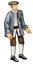
\includegraphics{../data/images/units/Unit0.png}} & Free Colonist & 0 & 3 & 0 & 1\\
%% \raisebox{-10mm}{
\includegraphics{../data/images/units/Unit27.png}} & Indentured Servant & -1 & 3 & 0 & 1\\
%% \raisebox{-10mm}{
\includegraphics{../data/images/units/Unit28.png}} & Petty Criminal & -2 & 3 & 0 & 1\\
%% \raisebox{-10mm}{
\includegraphics{../data/images/units/Unit1.png}} & Master Farmer & 1 & 3 & 0 & 1\\
%% \raisebox{-10mm}{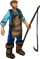
\includegraphics{../data/images/units/Unit2.png}} & Expert Fisherman & 1 & 3 & 0 & 1\\
%% \end{longtable}

\hypertarget{Skills and Education}{\subsection{Skills and Education}}

In FreeCol, your colonists come from all walks of life. Some are
unskilled \hyperlink{Petty Criminal}{Petty Criminals}, who are
deported to the colonies. Others are \hyperlink{Indentured
Servant}{Indentured Servants}, or \hyperlink{Free Colonist}{Free
Colonists} with moderate skills. Still others are masters of their
craft, experts at their trade or profession, who were educated at the
Royal College in Europe. If you have enough gold, you can recruit
units directly from the Royal College.

Not all skills, however, can be learned in Europe.
\hyperlink{Sugar}{Sugar}, \hyperlink{Cotton}{Cotton} and
\hyperlink{Tobacco}{Tobacco}, as well as \hyperlink{Furs}{Furs} are
apparently unknown in Europe. Thus, \hyperlink{Master Sugar
Planter}{Master Sugar Planters}, \hyperlink{Master Cotton
Planter}{Master Cotton Planters}, \hyperlink{Master Tobacco
Planter}{Master Tobacco Planters}, as well as the \hyperlink{Expert
Fur Trapper}{Expert Fur Trappers}, can not be recruited in Europe.

At the beginning of the game, these skills can only be learned at
Indian Settlements, or through experience. If you put a Free Colonist
to work outside of the colony for a long time without changing his
work assignment, he may learn the necessary skill and become an
expert. This does not work for the more complicated jobs within the
colony, however. 

As soon as you construct a \hyperlink{Schoolhouse}{Schoolhouse}, you
can place a master craftsman in the Schoolhouse in order to teach
other free colonists his skill. Petty Criminals and Indentured
Servants can not be directly upgraded to master craftsmen.  However, a
Petty Criminal may become an Indentured Servant, and an Indentured
Servant may become a Free Colonist through education. Petty Criminals
may also become Indentured Servants, and Indentured Servants may also
become Free Colonists by winning a battle.

Indian units are more productive than free colonists when working
outside of the colony, and less productive when working inside a
building. Indian units can not become free colonists through
education, but all Indian units become free colonists as soon as
\hyperlink{Bartolome de las Casas}{Bartolom\'e de las Casas} joins
the \hyperlink{Continental Congress}{Continental Congress}.

\hyperlink{Scout}{Scouts} can explore the New World and enter Indian
Settlements in order to speak with the tribal chiefs. A scout entering
an Indian Settlement may become a \hyperlink{Seasoned Scout}{Seasoned
Scout} through experience. A colonist investigating a \hyperlink{Lost
City Rumours}{Lost City Rumours} may also be upgraded to a Seasoned
Scout, unless that unit already has another skill.


\hypertarget{Combat}{\subsection{Combat}}

A tile can only be occupied by units of a single Player. If a unit of
another Player attempts to enter that tile, combat ensues. The combat
mechanism of FreeCol is very simple: Each unit has an attack strength
and a defence strength. Attack bonuses and defence bonuses granted by
terrain, fortifications or \hyperlink{Founding Fathers}{Founding
Fathers} are added to the base values of the units. If the attack
value of the attacker is greater than the defence value of the
defender, the attacker wins. Otherwise the defender wins. If a tile is
occupied by more than one unit, the attacker will fight against the
defender with the strongest defence.

Most units that win a battle may be promoted, and all units that lose
a battle will always be captured, demoted, damaged or destroyed. A
\hyperlink{Petty Criminal}{Petty Criminal} may be promoted to an
\hyperlink{Indentured Servant}{Indentured Servant}, and an Indentured
Servant may be promoted to a \hyperlink{Free Colonist}{Free
Colonist}. A Free Colonist may be promoted to a \hyperlink{Veteran
Soldier}{Veteran Soldier}, which in turn may be promoted to a
\hyperlink{Colonial Regular}{Colonial Regular}, but only after the
\hyperlink{Declaration of Independence}{Declaration of Independence}.

A Dragoon that loses a battle will be demoted to a Soldier, and a
Soldier that loses a battle will be demoted to an unarmed colonist. An
unarmed colonist that loses a battle is either captured, if the
attacker is a European Player, or slaughtered, if the attacker is a
Native Player. \hyperlink{Wagon Train}{Wagon Trains} and
\hyperlink{Treasure Train}{Treasure Trains} may also be captured by a
European Player and destroyed by a Native Player. Native units that
lose a battle are always slaughtered.

\hyperlink{Naval Units}{Naval units} and
\hyperlink{Artillery}{Artillery} can not be promoted. A beaten
artillery unit becomes a \hyperlink{Damaged Artillery}{Damaged
Artillery}, which can not be repaired and will be destroyed if it
loses another battle. Ships are either sunk or damaged when they lose
a battle. In either case all units and cargo aboard the ship are lost,
and the ship automatically returns to the nearest repair
location. This may be one of your colonies with a
\hyperlink{Drydock}{Drydock} or the \hyperlink{Home Port}{Home Port}.

The \hyperlink{Frigate}{Frigate}, the \hyperlink{Man of War}{Man of
War} and the \hyperlink{Privateer}{Privateer} have the ability to
capture the goods aboard an enemy ship they have bested in
battle. Naturally, they can not take more cargo than their holds will
allow.

Naval units can also attack colonies on coastal tiles, although their
chance of success is not very high. And colonies with a
\hyperlink{Fort}{Fort} or \hyperlink{Fortress}{Fortress} will
automatically fire at enemy ships on adjacent ocean tiles.


\hypertarget{Continental Congress}{\section{The Continental Congress}}

As the player generates \hyperlink{Liberty Bells}{Liberty Bells},
\hypertarget{Founding Fathers}{\textbf{Founding Fathers}} are elected
to the {\textbf{Continental Congress}}. The Founding Fathers are
historical figures who played a more or less important part in the
conquest of the New World. Each Founding Father grants the player a
new bonus or ability, or causes a certain event to occur, much like
the ``Wonders of the World'' in the Civilization series. At the
beginning of the game, you will need only a few Liberty Bells to elect
a Founding Father to the Continental Congress, but as the game
progresses this number may increase to many hundred Bells.

\Father{Adam Smith} (1723--1790), better known as the Father of Modern
Economics, penned several texts pertaining to Economic theory,
including, ``The Wealth of Nations'' his most famous text. As soon as
Adam Smith joins the Continental Congress, the player is allowed to
build factories, which produce 1.5 units of manufactured goods for
each unit of raw material consumed. \Wikipedia{Adam_Smith}

\Father{Jacob Fugger II} (1459--1525) was an extremely wealthy German
merchant and banker who amassed a fortune with family partnerships and
stock holdings in the mining industries. As soon as Jacob Fugger joins
the Continental Congress, all \hyperlink{Boycotts}{Boycotts} currently
in effect are dropped. \Wikipedia{Jacob_Fugger}

\Father{Peter Minuit} (1580--1638) bought what later became known as
Manhattan Island from Native Americans for about 60 Dutch guilders. He
later colonized the Delware Bay area as well. As soon as Peter Minuit
is elected to the Continental Congress, the Indians no longer demand
payment for their land. \Wikipedia{Peter_Minuit}

\Father{Peter Stuyvesant} (1592--1672) was appointed Governor General
of the New Netherlands, which, after a British invasion he could not
stop, became New York. With the election of Peter Stuyvesant, the
construction of \hyperlink{Custom House}{custom houses} becomes
possible. \Wikipedia{Peter_Stuyvesant}

\Father{Jan de Witt} (1625--1672) was a great Dutch statesmen.  He
represented the merchants and a encouraged industry and commerce. He
also negotiated several important treaties for the Dutch to end wars
with England. As soon as Jan de Witt is a member of the Continental
Congress, trade with foreign colonies becomes possible.
\Wikipedia{Jan_de_Witt}

\Father{Ferdinand Magellan} (1480--1521) was one of the greatest
explorers to navigate the globe. Magellan was first to circumnavigate
the globe and cross the Pacific Ocean. Magellan's election to the
Continental Congress increases the movement of all naval vessels by
one, and the time to sail between Europe and the New World is
reduced. \Wikipedia{Ferdinand_Magellan}

\FFather{Francisco de Coronado}{Francisco V\'azquez de Coronado}
(1510--1554) was the first European explorer to see the Grand
Canyon. Though he never found the golden cities he searched for, his
mapping of the area now called the Southwestern US was important to
further exploration. As soon as Francisco de Coronado joins the
Continental Congress, all existing colonies become visible on the
map. \Wikipedia{Francisco_V�zquez_de_Coronado}

\Father{Hernando de Soto} (1496--1542) was the first European to
explore Florida and the southeastern US.  He also held a prominent
role in conquests of Central America. If Hernando de Soto is a member
of the Continental Congress, the exploration of \hyperlink{Lost City
Rumours}{Lost City Rumours} always yields a positive result, and all
units have an extended sight radius. \Wikipedia{Hernando_de_Soto_(explorer)}

\Father{Henry Hudson} (1565--1611) was an English navigator who
explored and mapped a large area of the northeastern North American
continent.  Many waterways in that region are named in his honour. His
original goal was to find the famed Northwest Passage. The election of
Henry Hudson to the Continental Congress doubles the output of all
\hyperlink{Expert Fur Trapper}{Fur Trappers}. \Wikipedia{Henry_Hudson}

\Father{Robert La Salle} (1643--1687) was the first European to travel
the length of the Mississippi river, while on a mission to set up
numerous trading posts along its banks.  He later claimed the whole
basin as Louisiana in honor of the French King. Later, he explored
several of the Great Lakes. If Robert La Salle is a member of the
Continental Congress, all colonies gain a stockade as soon as their
population reaches three colonists. \Wikipedia{Robert_La_Salle}

\FFather{Hernan Cortes}{Hern\'an Cort\'es} (1485--1547) was a famed Spanish
conquistador who overthrew the Aztec Empire and claimed Mexico for
Spain. As soon as Hern\'an Cort\'es joins the Continental Congress,
conquered native settlements always yield treasure (and in greater
abundance) and the King's \hyperlink{Galleon}{galleons} transport it
free of charge. \Wikipedia{Hernan_Cortes}

\Father{George Washington} (1732--1799) was the general who lead the
colonial army to victory over the British to gain independence for the
colonies. This victory and his leadership led to his being named the
new nation's first President. If George Washington is a member of the
Continental Congress, any soldier or dragoon who wins a combat is
automatically upgraded to the next possible
level. \Wikipedia{George_Washington}

\Father{Paul Revere} (1734--1818) was the famed rider of colonial
America who mounted his horse and rode through the countryside
alerting colonists that British soldiers were coming. He was captured
during the ride and later released when his captors believed they were
in grave danger and their prisoner might slow them down. With Paul
Revere a member of the Continental Congress, a colonist automatically
takes up any stockpiled muskets and defends an otherwise undefended
colony if it is attacked. \Wikipedia{Paul_Revere}

\Father{Francis Drake} (1542--1596) was a great English sea captain,
the first Englishman to circumnavigate the globe and a hero in the
fights against the Spanish Armada. The presence of Francis Drake in
the Continental Congress increases the combat strength of all
Privateers by 50\%. \Wikipedia{Francis_Drake}

\Father{John Paul Jones} (1741--1792) was hailed as a great sea
captain in America, and uttered the famous words "Sir, I have not yet
begun to fight" while fighting the British at sea. He later watched
his ship sink to the bottom of the ocean from the deck of a British
vessel. As soon as John Paul Jones is elected to the Continental
Congress, a \hyperlink{Frigate}{Frigate} is added to your colonial
navy for free. \Wikipedia{John_Paul_Jones}

\Father{Thomas Jefferson} (1743--1826), a powerful voice of
patriotism, was credited with writing the Declaration of
Independence. He later became the 3rd President of the US. The
election of Thomas Jefferson to the Continental Congress increases
Liberty Bell production in colonies by
50\%. \Wikipedia{Thomas_Jefferson}

\Father{Pocahontas} (1595--1617) was a peacemaker between early
Jamestown settlers and the Native Americans. She is credited with
sending food and other supplies to starving colonists there during
harsh times.  She later converted to Christianity and married an
Englishman.  When Pocahontas joins the Continental Congress, all
tension levels between you and natives are removed and Indian alarm is
generated half as fast. \Wikipedia{Pocahontas}

\Father{Thomas Paine} (1737--1809) inspired colonists with his pen at
the urging of Benjamin Franklin. He published a pamphlet, "Common
Sense", guiding the thoughts of patriots all over the colonies. The
election of Thomas Pain to the Continental Congress increases Liberty
Bell production in all your colonies by the value of the current
\hyperlink{Taxes}{tax rate}. \Wikipedia{Thomas_Paine}

\FFather{Simon Bolivar}{Sim\'on Bol\'{\i}var} (1783--1830) is remembered as a great
leader in the struggle for South American independence from
Spain. Bol\'{\i}var freed what is now Venezuela and later became its
first President. When Sim\'on Bol\'{\i}var joins the Continental
Congress, the Sons of Liberty membership in all existing colonies is
increased by 20\%. \Wikipedia{Simon_Bolivar}

\Father{Benjamin Franklin} (1706--1790), a heavy contributor to the
Declaration of Independence, was one of the voices of the
Revolution. He traveled extensively between Europe and the colonies,
and gained the support of the French in the war. As soon as Benjamin
Franklin is elected to the Continental Congress, the King's foreign
wars no longer have effect on relationships in the New World, and
Europeans in the New World always offer peace in
negotiations. \Wikipedia{Benjamin_Franklin}

\Father{William Brewster} (1567--1644) was the Puritan leader of the
Plymouth colony in New England. As soon as William Brewster joins the
Continental Congress, criminals or indentured servants no longer
appear on the docks and you can select which immigrant in the
recruitment pool to move to the docks. \Wikipedia{William_Brewster_(Pilgrim)}

\Father{William Penn} (1644--1718), a close friend of the Duke of
York, was granted the land that is mostly Pennsylvania, Delaware, and
New Jersey. He governed the Quaker colony for several years to provide
a haven to fellow Quakers. The election of William Penn increases
cross production in all colonies by 50\%. \Wikipedia{William_Penn}

\FFather{Father Jean de Brebeuf}{Father Jean de Br\'ebeuf} (1593--1649) 
founded Quebec City in Canada, befriended the Huron Indians and
converted many to Christianity. He died at the hands of the Iroquois
who had finally defeated their enemy, the Hurons. With Jean de Brebeuf
a member of the Continental Congress, all missionaries function as
experts. \Wikipedia{Jean_de_Brebeuf}

\FFather{Juan de Sepulveda}{Juan Gin\'es de Sep\'ulveda} (1781--1872) 
was a Spanish theologian who spoke out for the conquest of Indian
lands and forced evangelization of the natives. The election of Juan
de Sepulveda to the Continental Congress increases the chance that a
subjugated Indian settlement will ``convert'' and join a
colony. \Wikipedia{Juan_Gines_de_Sepulveda}

\FFather{Bartolome de las Casas}{Bartolom\'e de las Casas}
(1474--1566) was a Catholic Priest who traveled the Indies converting
Indians and chastising Spain for their treatment of the Natives. When
Bartolom\'e de las Casas joins the Continental Congress, all existing
Indian converts become free
colonists. \Wikipedia{Bartolome_de_las_Casas}



\hypertarget{The Birth of a Nation}{\section{The Birth of a Nation}}

\hypertarget{Sons of Liberty}{\subsection{Sons of Liberty}}

At the beginning of the game, all your colonists will be
\hypertarget{Tories}{\textbf{Tory Loyalists}}, who support your
\hyperlink{Monarch}{Monarch} and are opposed to your policies. For
this reason, colonies with more than a certain number of tories (which
depends on the difficulty setting) suffer production penalties, which
may well threaten their survival.

\hyperlink{Liberty Bells}{Liberty Bells}, however, will turn these
Tories into \textbf{Sons of Liberty}, who support your
policies. Colonies in which more than 50\% of the population are Sons
of Liberty enjoy a production bonus, which is further increased as
soon as 100\% of the population become Sons of Liberty.


\hypertarget{Declaration of Independence}{\subsection{The Declaration
of Independence}}

As soon as 50\% of your entire population support the Sons of Liberty,
you can declare the independence of your colonies. Your
\hyperlink{Monarch}{Monarch} will not be amused and will send the
\hyperlink{Royal Expeditionary Force}{Royal Expeditionary Force} to
quell the insurrection. In order to gain independence, you must defeat
the Royal Expeditionary Force. The European enemies of your Monarch
may support your effort if you generate a sufficient number of Liberty
Bells after the War of Independence has begun.


\hypertarget{Copyright Notice}{\section{Copyright Notice}}
Copyright � 2006
\href{http://freecol.sourceforge.net/index.php?section=8}{The FreeCol
Team}.

This manual is free software; you may redistribute it and/or modify it
under the terms of the GNU General Public License as published by the
Free Software Foundation; either version 2, or (at your option) any
later version.

This is distributed in the hope that it will be useful, but without
any warranty; without even the implied warranty of merchantability or
fitness for a particular purpose. See the GNU General Public License
for more details.

A copy of the GNU General Public License is available on the World
Wide Web at \href{http://www.gnu.org/copyleft/gpl.html}{the GNU
General Public Licence}. You can also obtain it by writing to the Free
Software Foundation, Inc., 59 Temple Place - Suite 330, Boston, MA
02111--1307, USA.


\printindex

\end{document}
